
%----------------------------------------------------------------------------------------
%	PACKAGES AND DOCUMENT CONFIGURATIONS
%----------------------------------------------------------------------------------------

\documentclass{article}

\usepackage[version=3]{mhchem} % Package for chemical equation typesetting
\usepackage{siunitx} % Provides the \SI{}{} and \si{} command for typesetting SI units
\usepackage{graphicx} % Required for the inclusion of images
\usepackage{natbib} % Required to change bibliography style to APA
\usepackage{amsmath} % Required for some math elements 
\usepackage{amssymb}
\setlength\parindent{0pt} % Removes all indentation from paragraphs
\usepackage{hyperref}
\renewcommand{\labelenumi}{\alph{enumi}.} % Make numbering in the enumerate environment by letter rather than number (e.g. section 6)
\usepackage{xfrac}
%\usepackage{times} % Uncomment to use the Times New Roman font
\usepackage{nicefrac}
\usepackage{graphicx}
\usepackage{caption}
\usepackage{subcaption}
%----------------------------------------------------------------------------------------
%	DOCUMENT INFORMATION
%----------------------------------------------------------------------------------------

\title{Arm Kinematics and Control \\ Algorithm and Simulation \\ Project Necessity: Arm Version 1.0} % Title

\author{Haoran \textsc{Yu}} % Author name

\date{March 16 2016} % Date for the report

\begin{document}

\maketitle

This kinematic document is for Arm Version 1.0. The kinematic document includes math background on Forward Kinematics and Jacobian, and also control algorithm on Resolved Rates and Redundancy Resolution. Future development includes Task Priority Redundancy Resolution.

Nomenclature:
\begin{enumerate}
\item Bold text is for vector or matrix, unbold text is for scalar.
\item $^{i}A_{j}$: $A$ of $j$ defined in $i$.
\item Without specific notation, all the vectors and matrices are defined in the base frame/world frame. This means we omit superscript $^0$ in some occasions. 
\item $\begin{bmatrix}\mathbf{r}\times\end{bmatrix}$ is the cross product matrix of vector $\mathbf{r}$. \url{https://en.wikipedia.org/wiki/Cross_product}
\end{enumerate}

%----------------------------------------------------------------------------------------
%	SECTION 1 Forward Kinematics
%----------------------------------------------------------------------------------------

\section{Forward Kinematics}
The forward kinematics takes URDF input exported from Solidworks and the current joint configuration and calculates the homogeneous transformation matrices. Figure 1 shows the arm home configuration with four important coordinate system.
\begin{figure}[htbp]
  \centering
    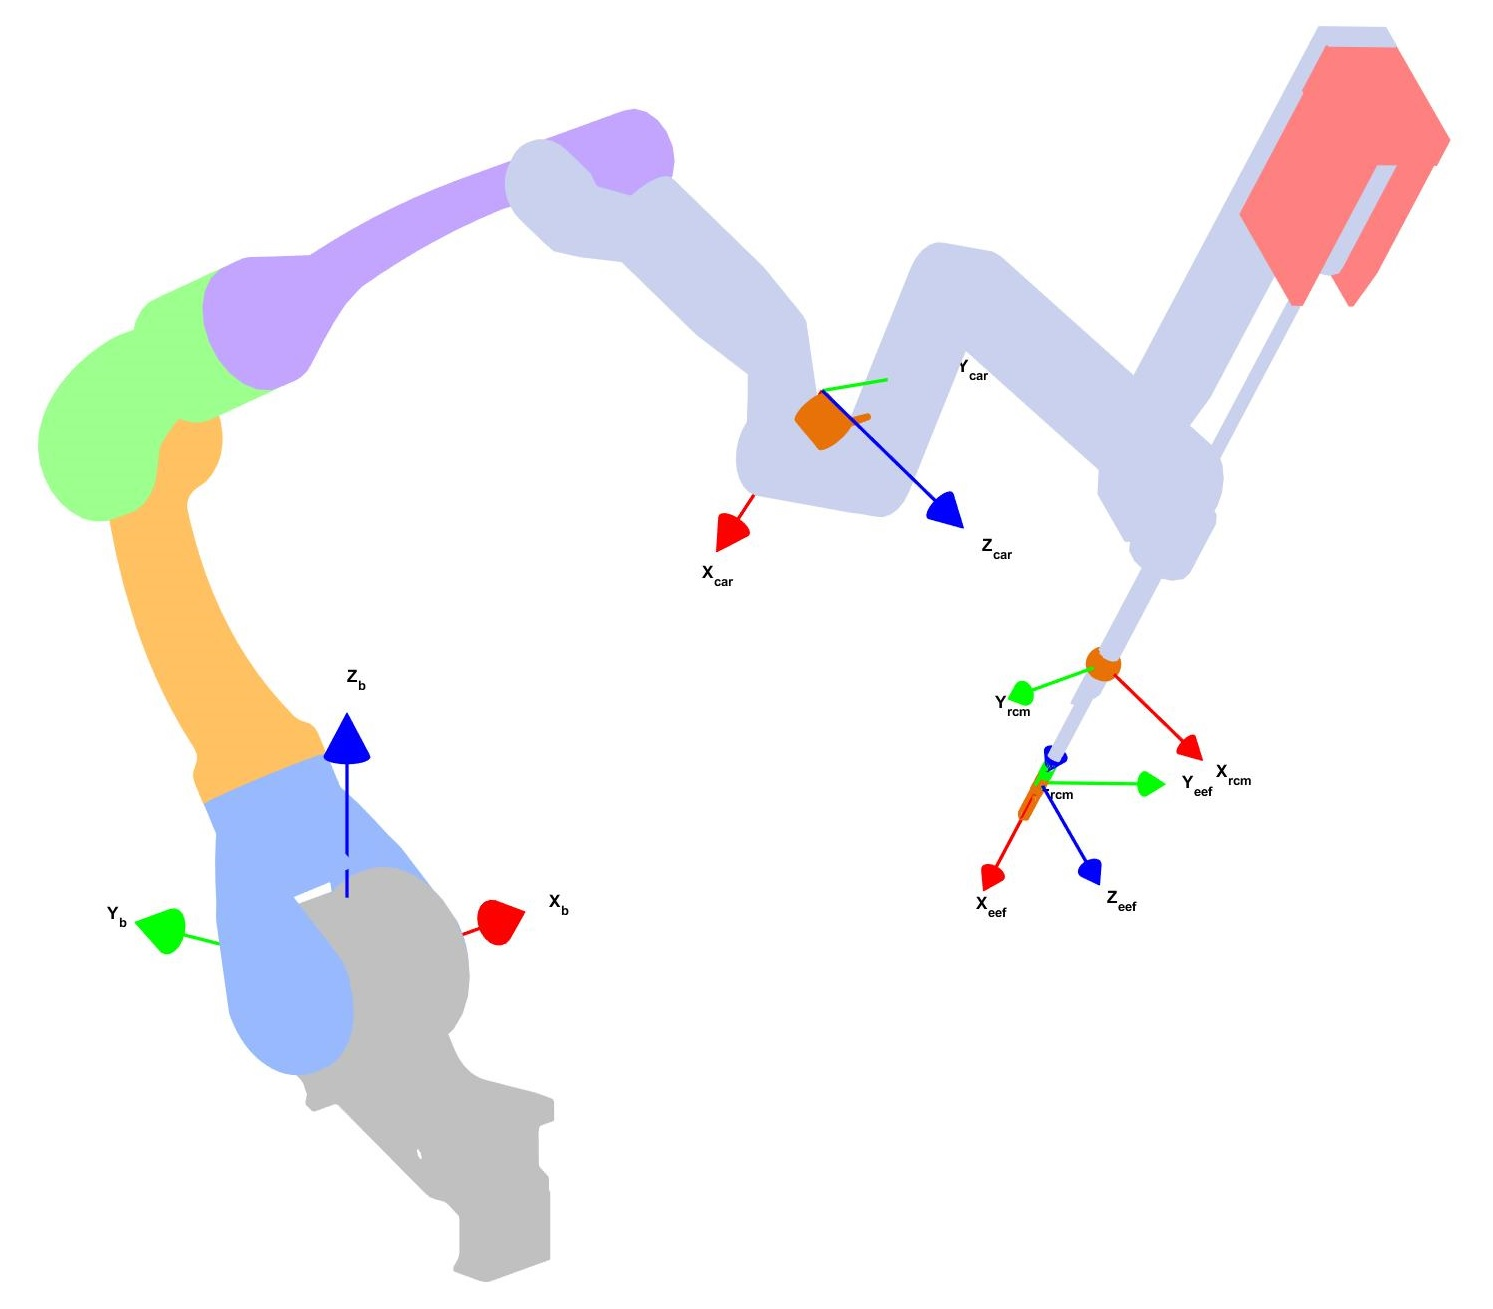
\includegraphics[width=1\columnwidth]{arm_home_config}
	\caption{Arm home configuration: generated in Matlab simulation}
\end{figure}
The joint information on $i^{th}$ coordinate from URDF export contains the origin $^{i-1}\mathbf{d}_i$ of axis defined in the parent frame $i-1$. It also provides roll pitch yaw rotation with respect to the fixed frame: $\alpha$, $\beta$, $\gamma$. And the URDF also defines the rotation axis of the active joint or translation axis for the prismatic joint: $^{i}\boldsymbol{\eta}_i$.
\begin{equation}
\begin{split}
Translation:&^{i-1}\mathbf{d}_i\\
Rotation:&\begin{bmatrix}
\alpha & \beta & \gamma
\end{bmatrix}\\
Axis:& ^{i}\boldsymbol{\eta}_i
\end{split}
\end{equation}
The joint value is given in a format of $11\times1$ vector $\mathbf{q}$. Since we have the coupling on pitch arm of the spherical arm, the RCM joint value is defined as $\mathbf{q}_{rcm}$ with a transformation matrix $\mathbf{A} \in \mathbb{R}^{[13\times11]}$
\begin{equation}
\begin{split}
&\mathbf{q}_{rcm} = \mathbf{A} \mathbf{q}\\
&\mathbf{A} = \begin{bmatrix}
\mathbf{I}_{6\times6} & \mathbf{0}_{6\times1} & \mathbf{0}_{6\times4}\\
\mathbf{0}_{3\times6} & \begin{bmatrix}1\\-1\\1\end{bmatrix} & \mathbf{0}_{3\times4}\\
\mathbf{0}_{4\times6} & \mathbf{0}_{4\times1} &\mathbf{I}_{4\times4}
\end{bmatrix}
\end{split}
\end{equation}
According to fixed frame rotation matrix, the rotation matix $^{i-1}\mathbf{R}_i$ is given by:
\begin{equation}
\begin{split}
Revolute: &^{i-1}\mathbf{R}_i = Rot(\hat{\mathbf{z}},\gamma)Rot(\hat{\mathbf{y}},\beta)Rot(\hat{\mathbf{x}},\alpha)Rot(^{i}\boldsymbol{\eta}_i,q_i)\\
Prismatic: &^{i-1}\mathbf{R}_i = Rot(\hat{\mathbf{z}},\gamma)Rot(\hat{\mathbf{y}},\beta)Rot(\hat{\mathbf{x}},\alpha)
\end{split}
\end{equation}
The translation part is given as following:
\begin{equation}
\begin{split}
Revolute: &^{i-1}\mathbf{p}_i = ^{i-1}\mathbf{d}_i\\
Prismatic: &^{i-1}\mathbf{p}_i = ^{i-1}\mathbf{d}_i + ^{i-1}\mathbf{R}_i(q_i {^{i}\boldsymbol{\eta}_i})
\end{split}
\end{equation}
The homogeneous transformation is then given by
\begin{equation}
^{i-1}\mathbf{T}_i = \begin{bmatrix} ^{i-1}\mathbf{R}_i &^{i-1}\mathbf{p}_i \\\mathbf{0}_{1\times3}&1\end{bmatrix}
\end{equation}
The homogeneous transformation with respect to the base frame is given by
\begin{equation}
^{0}\mathbf{T}_i = ^{0}\mathbf{T}_{i-1} {^{i-1}\mathbf{T}_i}
\end{equation}

%----------------------------------------------------------------------------------------
%	SECTION 2 Jacobian
%----------------------------------------------------------------------------------------

\section{Jacobian}
Most joints in our robotic arm is serial robot except for the spherical arm which has kinematic coupling. The overall arm Jacobian for all active and passive joints $\mathbf{J}_{all13} \in \mathbb{R}^{[6\times13]}$ from base to end-effector $\mathbf{p}_{eef}$ with 13 DoF joint input $\mathbf{q}_{rcm}$ ($i=1\cdots13$)
\begin{equation}
\mathbf{J}_{all13}(i) =  \begin{bmatrix}\hat{\mathbf{z}}_i \times (\mathbf{p}_{eef} - \mathbf{p}_i) \\ \hat{\mathbf{z}}_i \end{bmatrix}
\end{equation}
The overall arm Jacobian with only the active joints $\mathbf{q}$ ($i=1\cdots11$) is like this:
\begin{equation}
\mathbf{J}_{all} =  \mathbf{J}_{all13} * \mathbf{A}
\end{equation}
The overall arm Jacobian for all 11 DoF $\mathbf{J}_{all} \in \mathbb{R}^{[6\times11]}$ could be separate into $\mathbf{J}_{car5}$ for cartesian arm and $\mathbf{J}_{rcm}$ for spherical arm.
\begin{equation}
\mathbf{J}_{all} =  \begin{bmatrix} \mathbf{J}_{car5} & \mathbf{J}_{rcm} \end{bmatrix}
\end{equation}
%----------------------------------------------------------------------------------------
%----------------------------------------------------------------------------------------
%	SECTION 3 Resolved Rates
%----------------------------------------------------------------------------------------

\section{Resolved Rates}
Resolved rates algorithm is for controlling the robot with given desired end-effector configuration. No matter the end-effector configuration is defined in any kind of format (homogeneous transformation, quarternion or roll pitch yaw). Here we use homegeneous transformation matrix to define target tracking.

The reference configuration of end effector is $\mathbf{T}_{ref}$.
\begin{equation}
\mathbf{T}_{ref} = \begin{bmatrix}\mathbf{R}_{ref} & \mathbf{p}_{ref} \\ \mathbf{0}_{1\times3} & 1\end{bmatrix}
\end{equation}
The difference between current end effector configuration and the reference one.
\begin{equation}
\begin{split}
\mathbf{p}_{e} & = \mathbf{p}_{ref} - \mathbf{p}_{eef}\\
\mathbf{R}_{e} & = \mathbf{R}_{ref}  \mathbf{R}_{eef}^T
\end{split}
\end{equation}
Several variables defined for resolved rates algorithm.
\begin{enumerate}
\item $\Delta t$: discrete time step.
\item $\mathbf{v}_{max}$ and $\boldsymbol{\omega}_{max}$: maximum linear and angular velocity.
\item $p_{eps}$ and $\theta_{eps}$: Convergence criteria for translation and rotation. When error is within the criteria, we don't move the robot.
\item $n_t$ and $n_r$: These two defines the cycles before approaching the target with maximum velocity. Within the cycle, the end-effector twist starts to slow down.
\end{enumerate}
The end-effector linear velocity is given by following criteria.
\begin{equation}
\mathbf{v}_{eef} = \left\{\begin{matrix}
\mathbf{0}_{3\times1}, & |\mathbf{p}_{e} | < p_{eps} \\ 
\mathbf{p}_{e}/(n_t \Delta t), & p_{eps} \leqslant |\mathbf{p}_{e} | < n_t v_{max} \Delta t\\ 
v_{max} \mathbf{p}_e / |\mathbf{p}_e|, & |\mathbf{p}_{e} | \geqslant n_t v_{max} \Delta t
\end{matrix}\right.
\end{equation}
For rotation, we first need to convert rotation matrix to axis and angle of rotation.
\begin{equation}
\begin{split}
\theta_e & =\arccos((tr(\mathbf{R}_e)-1)/2)\\
\boldsymbol{\eta}_e &= \frac{1}{2}\begin{bmatrix} \mathbf{R}_e(3,2) - \mathbf{R}_e(2,3) \\ \mathbf{R}_e(1,3) - \mathbf{R}_e(3,1) \\ \mathbf{R}_e(2,1) - \mathbf{R}_e(1,2) \end{bmatrix}
\end{split}
\end{equation}
The angular velocity of end effertor is given as following.
\begin{equation}
\boldsymbol{\omega}_{eef} = \left\{\begin{matrix}
\mathbf{0}_{3\times1}, & |\boldsymbol{\theta}_{e} | < \theta_{eps} \\ 
\theta_e \boldsymbol{\eta}_e / (n_r \Delta t), &  \theta_{eps} \leqslant |\boldsymbol{\theta}_{e}| < n_r \omega_{max} \Delta t\\ 
\omega_{max} \boldsymbol{\eta}_e, & |\boldsymbol{\theta}_{e}| \geqslant n_r \omega_{max} \Delta t
\end{matrix}\right.
\end{equation}
So the end effector twist is given by
\begin{equation}
\mathbf{t}_{eef} = \begin{bmatrix} \mathbf{v}_{eef} \\ \boldsymbol{\omega}_{eef} \end{bmatrix}
\end{equation}
Differenct control mode and different task will require using different Jacobian and select different end effector. We take the 6DoF spherical arm as an example here. The Jacobian is the 6DoF RCM Jacobian $\mathbf{J}_{rcm}$. And without redundancy in the system, we will use tseu-do inverse to solve the desired joint velocity.
\begin{equation}
\dot{\mathbf{q}}_{6\cdots11} = \mathbf{J}_{rcm}^+ \mathbf{t}_{eef}
\end{equation}
The overall joint velocity
\begin{equation}
\dot{\mathbf{q}}_{1\cdots11} = \begin{bmatrix}\mathbf{0}_{1\cdots5} \\ \dot{\mathbf{q}}_{6\cdots11} \end{bmatrix}
\end{equation}
And the desired joint angle is given by
\begin{equation}
\mathbf{q}_{des} = \mathbf{q}_{cur} + \dot{\mathbf{q}} \Delta t
\end{equation}

The simulation of targeting the robot end effector is shown in the figure.
\begin{figure}
    \centering
    \begin{subfigure}[b]{0.454\textwidth}
        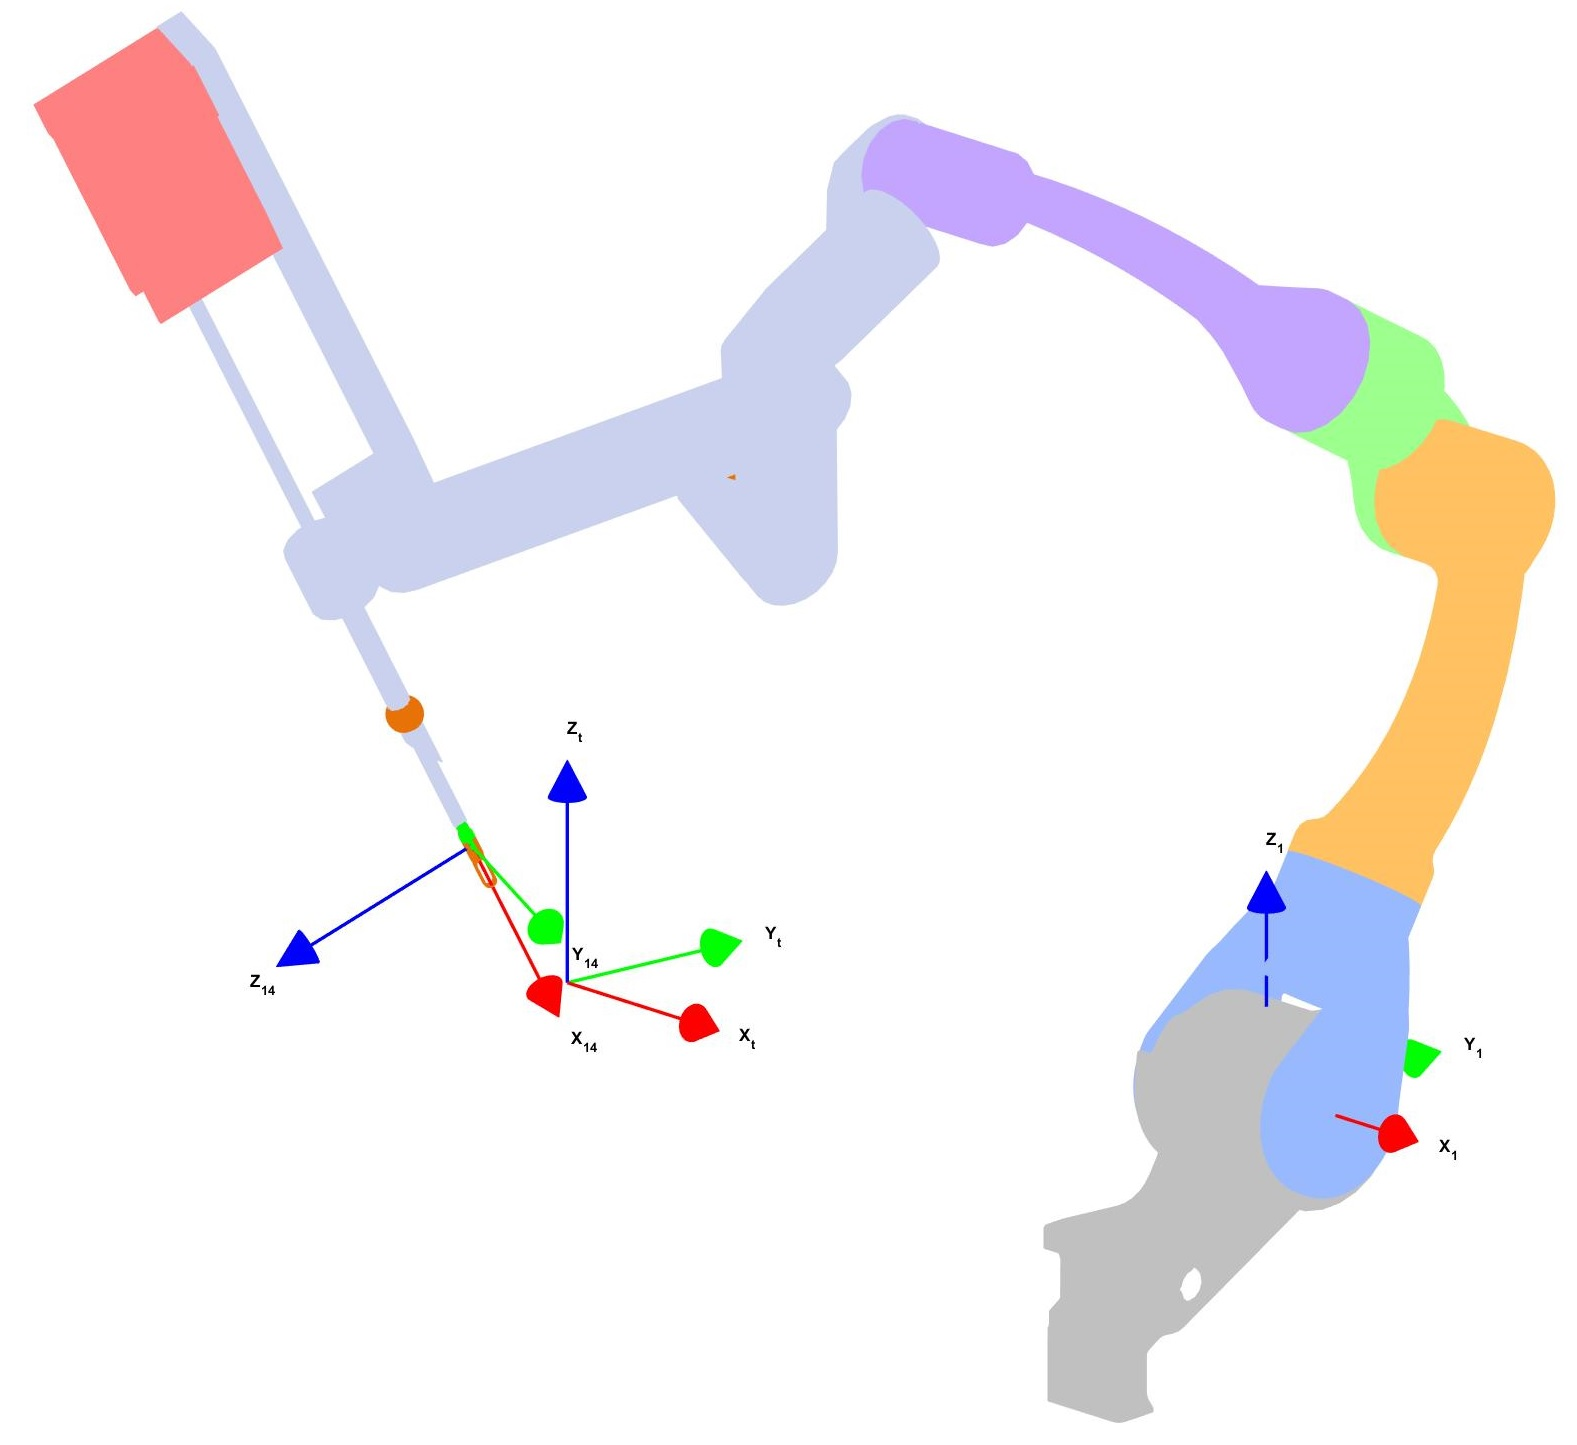
\includegraphics[width=\textwidth]{before_move}
        \caption{Before move}
        \label{fig:before_move}
    \end{subfigure}
	~
    \begin{subfigure}[b]{0.45\textwidth}
        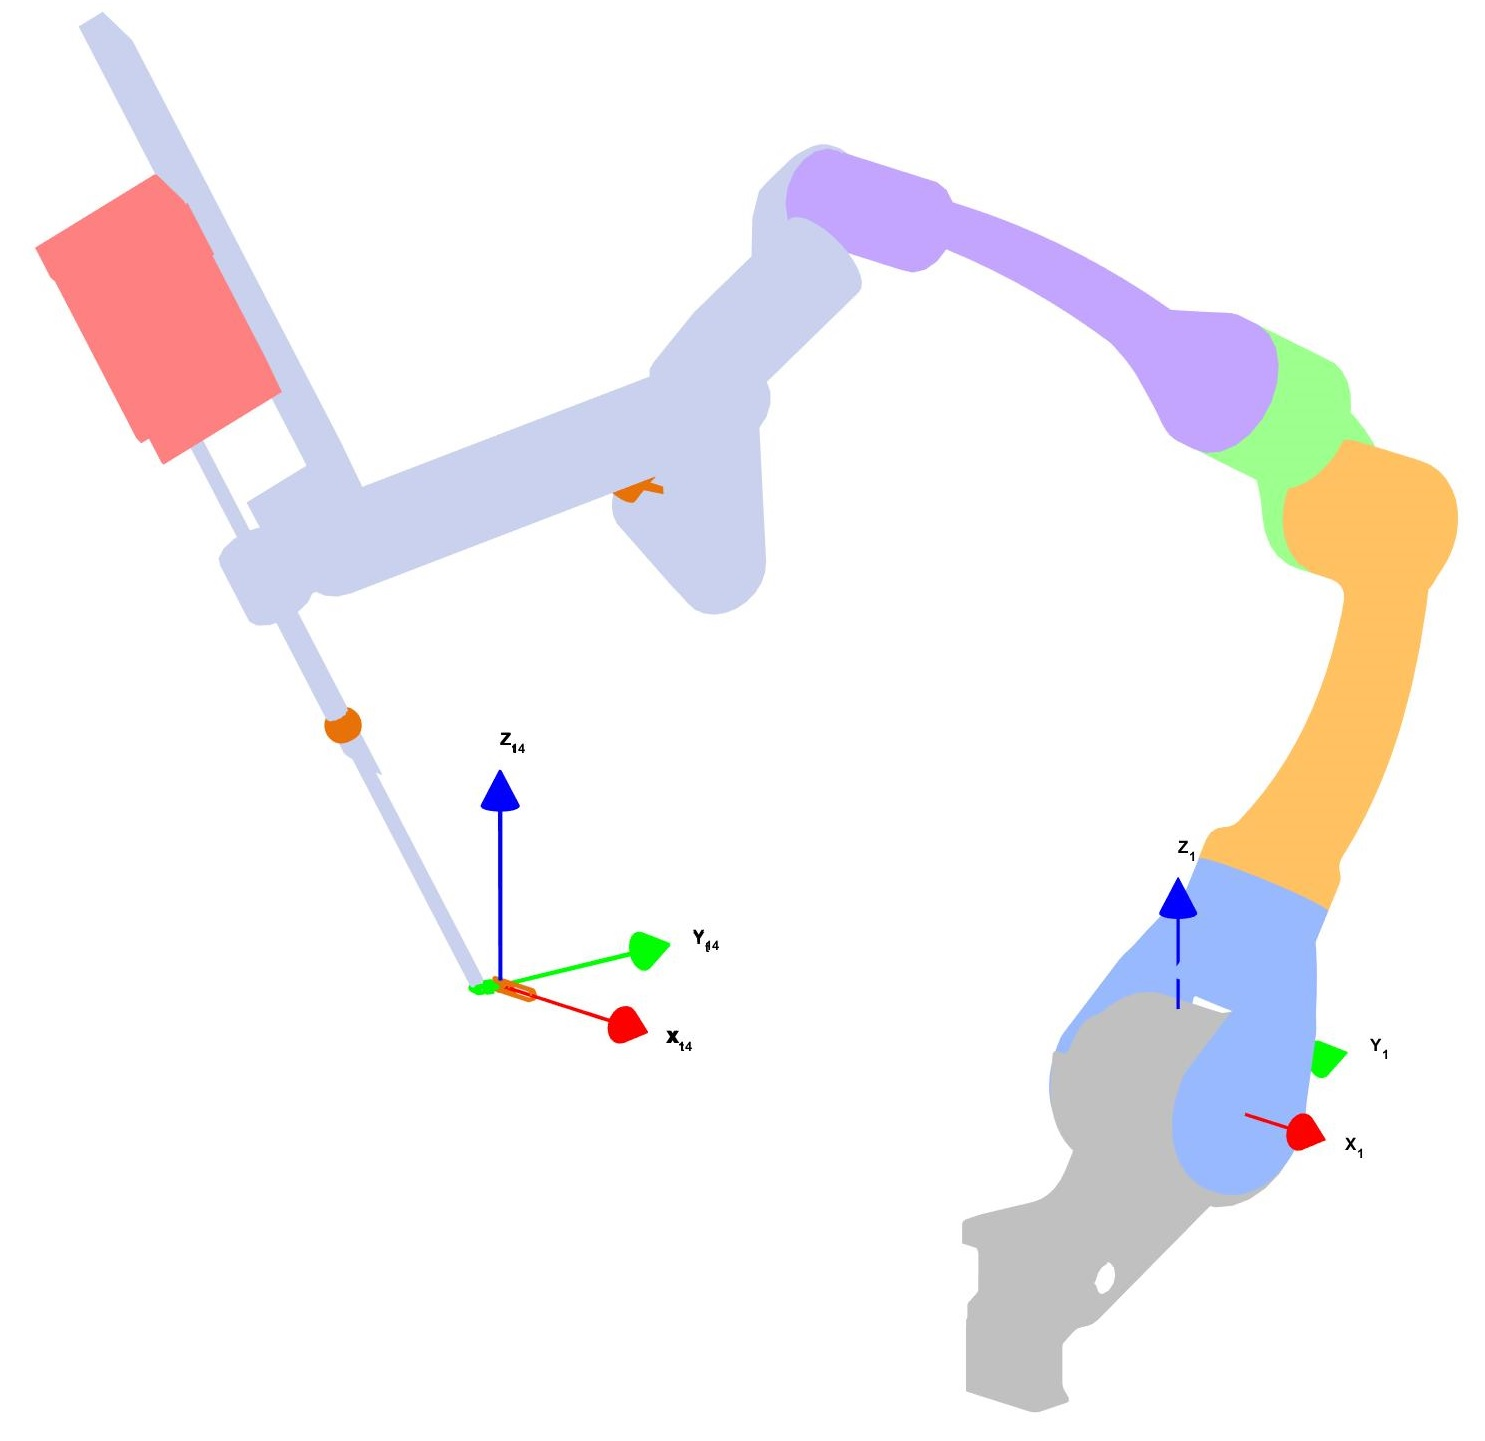
\includegraphics[width=\textwidth]{after_move}
        \caption{After move}
        \label{fig:after_move}
    \end{subfigure}
\end{figure}

\end{document}